\documentclass[10pt,fleqn]{article}
\newcommand{\name}[1]{\def\psettitlename{#1}}
\newcommand{\course}[1]{\def\psettitlecourse{#1}}
\newcommand{\rsection}[1]{\def\psettitlersection{#1}}
\newcommand{\psetnum}[1]{\def\psettitlepsetnum{#1}}
% \usepackage[journal=rsc]{chemstyle}
% \usepackage{mhchem}
\usepackage{amsmath}
\usepackage{amssymb}
\usepackage{amsfonts}
\usepackage{esint}
\usepackage{bbm}
\usepackage{amscd}
\usepackage{picinpar}
\usepackage[pdftex]{graphicx}
\usepackage{indentfirst}
\usepackage{wrapfig}
\usepackage{units}
\usepackage{textcomp}
\usepackage[utf8x]{inputenc}
\usepackage{feyn}
\usepackage{feynmp}
\DeclareGraphicsRule{*}{mps}{*}{}
\newcommand{\ud}{\mathrm{d}}
\newcommand{\ue}{\mathrm{e}}
\newcommand{\ui}{\mathrm{i}}
\newcommand{\res}{\mathrm{Res}}
\newcommand{\Tr}{\mathrm{Tr}}
\newcommand{\dsum}{\displaystyle\sum}
\newcommand{\dprod}{\displaystyle\prod}
\newcommand{\dlim}{\displaystyle\lim}
\newcommand{\dint}{\displaystyle\int}
\newcommand{\fsno}[1]{{\!\not\!{#1}}}
\newcommand{\eqar}[1]
{
  \begin{align*}
    #1
  \end{align*}
}
\newcommand{\texp}[2]{\ensuremath{{#1}\times10^{#2}}}
\newcommand{\dexp}[2]{\ensuremath{{#1}\cdot10^{#2}}}
\newcommand{\eval}[2]{{\left.{#1}\right|_{#2}}}
\newcommand{\paren}[1]{{\left({#1}\right)}}
\newcommand{\lparen}[1]{{\left({#1}\right.}}
\newcommand{\rparen}[1]{{\left.{#1}\right)}}
\newcommand{\abs}[1]{{\left|{#1}\right|}}
\newcommand{\sqr}[1]{{\left[{#1}\right]}}
\newcommand{\crly}[1]{{\left\{{#1}\right\}}}
\newcommand{\angl}[1]{{\left\langle{#1}\right\rangle}}
\newcommand{\tpdiff}[4][{}]{{\paren{\frac{\partial^{#1} {#2}}{\partial {#3}{}^{#1}}}_{#4}}}
\newcommand{\tpsdiff}[4][{}]{{\paren{\frac{\partial^{#1}}{\partial {#3}{}^{#1}}{#2}}_{#4}}}
\newcommand{\pdiff}[3][{}]{{\frac{\partial^{#1} {#2}}{\partial {#3}{}^{#1}}}}
\newcommand{\diff}[3][{}]{{\frac{\ud^{#1} {#2}}{\ud {#3}{}^{#1}}}}
\newcommand{\psdiff}[3][{}]{{\frac{\partial^{#1}}{\partial {#3}{}^{#1}} {#2}}}
\newcommand{\sdiff}[3][{}]{{\frac{\ud^{#1}}{\ud {#3}{}^{#1}} {#2}}}
\newcommand{\tpddiff}[4][{}]{{\left(\dfrac{\partial^{#1} {#2}}{\partial {#3}{}^{#1}}\right)_{#4}}}
\newcommand{\tpsddiff}[4][{}]{{\paren{\dfrac{\partial^{#1}}{\partial {#3}{}^{#1}}{#2}}_{#4}}}
\newcommand{\pddiff}[3][{}]{{\dfrac{\partial^{#1} {#2}}{\partial {#3}{}^{#1}}}}
\newcommand{\ddiff}[3][{}]{{\dfrac{\ud^{#1} {#2}}{\ud {#3}{}^{#1}}}}
\newcommand{\psddiff}[3][{}]{{\frac{\partial^{#1}}{\partial{}^{#1} {#3}} {#2}}}
\newcommand{\sddiff}[3][{}]{{\frac{\ud^{#1}}{\ud {#3}{}^{#1}} {#2}}}
\usepackage{fancyhdr}
\usepackage{multirow}
\usepackage{fontenc}
% \usepackage{tipa}
\usepackage{ulem}
\usepackage{color}
\usepackage{cancel}
\newcommand{\hcancel}[2][black]{\setbox0=\hbox{#2}%
  \rlap{\raisebox{.45\ht0}{\textcolor{#1}{\rule{\wd0}{1pt}}}}#2}
\pagestyle{fancy}
\setlength{\headheight}{67pt}
\fancyhead{}
\fancyfoot{}
\fancyfoot[C]{\thepage}
\fancyhead[R]
{
  \psettitlename \\
  \psettitlecourse{} Problem Set \psettitlepsetnum \\
  \ifx\psettitlersection\empty
  \else
  Recitation Section \psettitlersection
  \fi
}
\renewcommand{\footruleskip}{0pt}
\renewcommand{\headrulewidth}{0.4pt}
\renewcommand{\footrulewidth}{0pt}
\addtolength{\hoffset}{-1.3cm}
\addtolength{\voffset}{-2cm}
\addtolength{\textwidth}{3cm}
\addtolength{\textheight}{2.5cm}
\renewcommand{\footskip}{10pt}
\setlength{\headwidth}{\textwidth}
\setlength{\headsep}{20pt}
\setlength{\marginparwidth}{0pt}
\parindent=0pt
\psetnum{4}
\course{Physics 251b}
\rsection{1}
\name{Yichao Yu}
\renewcommand{\thesection}{\arabic{section}.}
\renewcommand{\thesubsection}{(\alph{subsection})}
\renewcommand{\thesubsubsection}{\roman{subsubsection}.}

\begin{document}
\section{}
Hamiltonian
\eqar{
  H=&\frac{1}{2m}\paren{\vec p-\frac{q\vec A}{c}}^2
  \intertext{Interaction term}
  V=&\frac{q}{2mc}\paren{-\vec p\cdot\vec A-\vec A\cdot\vec p+\frac{qA^2}{c}}\\
  =&\frac{q}{2mc}\paren{\ui\hbar\nabla\cdot\vec A-2\vec A\cdot\vec p+\frac{qA^2}{c}}
  \intertext{Scattering wavefunction given by Born approximation}
  \langle x|\psi^{(+)}\rangle=&\langle x|\vec k\rangle-\frac{2m}{\hbar^2}\int\ud^3x'\frac{\ue^{\ui\vec k\paren{\vec x - \vec x'}}}{4\pi\abs{\vec x-\vec x'}}\langle x'|V|\vec k\rangle\\
  =&\langle x|\vec k\rangle-\frac{q}{\hbar^2c}\int\ud^3x'\frac{\ue^{\ui\vec k\paren{\vec x - \vec x'}}}{4\pi\abs{\vec x-\vec x'}}\langle x'|\paren{\ui\hbar\nabla\cdot\vec A-2\vec A\cdot\vec p+\frac{qA^2}{c}}|\vec k\rangle\\
  =&\langle x|\vec k\rangle-\frac{q}{\hbar^2c}\int\ud^3x'\frac{\ue^{\ui\vec k\paren{\vec x - \vec x'}}}{4\pi\abs{\vec x-\vec x'}}\langle x'|\paren{\ui\hbar\nabla\cdot\vec A'-2\hbar\vec A'\cdot\vec k+\frac{qA'^2}{c}}|\vec k\rangle\\
  \approx&\langle x|\vec k\rangle-\frac{q}{\hbar c}\frac{\ue^{\ui kr}}{4\pi r}\int\ud^3x'\ue^{-\ui\vec k'\cdot\vec x'}\paren{\ui\nabla\cdot\vec A'-2\vec A'\cdot\vec k+\frac{qA'^2}{\hbar c}}\langle x'|\vec k\rangle\\
  =&\langle x|\vec k\rangle-\frac{q}{\paren{2\pi}^{3/2}\hbar c}\frac{\ue^{\ui kr}}{4\pi r}\int\ud^3x'\ue^{\ui\paren{\vec k - \vec k'}\cdot\vec x'}\paren{\ui\nabla\cdot\vec A'-2\vec A'\cdot\vec k+\frac{qA'^2}{\hbar c}}\\
}
\section{}
The plane wave function,
\eqar{
  \ue^{\ui\vec k\cdot\vec r}=&\ue^{\ui kr\cos\varphi}\\
  =&\sum_{m=-\infty}^{\infty}c_n\paren{kr}\ue^{\ui m\varphi}
  \intertext{Integrate both side with $\ue^{-\ui m\varphi}$}
  c_m\paren{kr}=&\frac{1}{2\pi}\int_0^{2\pi}\ue^{\ui kr\cos\varphi}\ue^{-\ui m\varphi}\ud\varphi\\
  =&\ui^mJ_m\paren{kr}
}
where $J_m$ is the Bessel function.

At $\rho\rightarrow\infty$ the wavefunction
\eqar{
  \psi^{(+)}\approx&f(\varphi)\frac{\ue^{\ui k\rho}}{\sqrt{\rho}}
}

Expanding $f(\varphi)$
\eqar{
  f(\varphi)=&\frac{1}{\sqrt{k}}\sum_{m=-\infty}^{\infty}\ue^{\ui\delta_m}\sin\delta_m\ue^{\ui m\varphi}
}

Total cross section
\eqar{
  \sigma_{tot}=&\int\ud\varphi\abs{\frac{1}{\sqrt{k}}\sum_{m=-\infty}^{\infty}\ue^{\ui\delta_m}\sin\delta_m\ue^{\ui m\varphi}}^2\\
  =&\frac{1}{k}\int\ud\varphi\sum_{m,m'=-\infty}^{\infty}\ue^{\ui\delta_m}\sin\delta_m\ue^{\ui\delta_m}\sin\delta_{m'}\ue^{-\ui m'\varphi}\ue^{\ui m\varphi}\\
  =&\frac{2\pi}{k}\sum_{m=-\infty}^{\infty}\sin^2\delta_m
}
Optical theorem,
\eqar{
  \Im\paren{f(0)}=&\Im\paren{\frac{1}{\sqrt{k}}\sum_{m=-\infty}^{\infty}\ue^{\ui\delta_m}\sin\delta_m}\\
  =&\frac{1}{\sqrt{k}}\sum_{m=-\infty}^{\infty}\sin^2\delta_m\\
  =&\frac{\sqrt{k}}{2\pi}\sigma_{tot}
}

\section{}
\section{}
\subsection{}
Since there's only two plain wave solutions.
\eqar{
  \psi^{(+)}=&\frac{1}{\sqrt{2\pi}}\paren{\ue^{\ui kx}+f(sign(x))\ue^{\ui k\abs{x}}}
}

\subsection{}
From the conservation of probability density,
the in-coming and out-going wave must have the same amplitude.
Therefore, there can only be a phase shift between them.

Using the boundary condition, the wavefunction for $0 < x < a$ is,
\eqar{
  \psi=&A\paren{\ue^{\ui k'x}-\ue^{-\ui k'x}}
}
where $k'=\sqrt{k^2+2mV_0}$ and for $x \geqslant a$ is
\eqar{
  \psi=&\ue^{\ui\paren{kx+\delta}}-\ue^{-\ui\paren{kx+\delta}}
}
To satisfy the continuity condition at $x=a$
\eqar{
  A\ue^{\ui k'a}-A\ue^{-\ui k'a}=&\ue^{\ui\paren{ka+\delta}}-\ue^{-\ui\paren{ka+\delta}}\\
  Ak'\ue^{\ui k'a}+Ak'\ue^{-\ui k'a}=&k\ue^{\ui\paren{ka+\delta}}+k\ue^{-\ui\paren{ka+\delta}}\\
  A\sin k'a=&\sin\paren{ka+\delta}\\
  Ak'\cos k'a=&k\cos\paren{ka+\delta}\\
  \delta=&\arctan\paren{\frac{k}{k'}\tan k'a}-ka
}
Scattering coefficient
\eqar{
  \abs{1-\ue^{2\ui\delta}}^2=&4\sin^2\delta
}
Since $\arctan\paren{\frac{k}{k'}\tan k'a}$ is in $\sqr{-\dfrac\pi2, \dfrac\pi2}$,
$\delta$ can be smaller than $-\dfrac\pi2$ if $ka$ is large, in which case the
scattering coefficient will have maxima.
\section{}
For hard sphere, the boundary condition is
\eqar{
  A_l\paren{R}=&0
}
where $A_l$ is the radial wave function of the $l$th partial wave.
\eqar{
  A_l\paren{r}=&\ue^{\ui\delta_l}j_l(kr)\cos\delta_l-n_l(kr)\sin\delta_l
}
\eqar{
  \tan\delta_l=&\frac{j_l\paren{kR}}{n_l\paren{kR}}
}
For $k=\dfrac1R$
\eqar{
  \tan\delta_l=&\frac{j_l\paren{1}}{n_l\paren{1}}
}
Differencial cross section
\begin{center}
  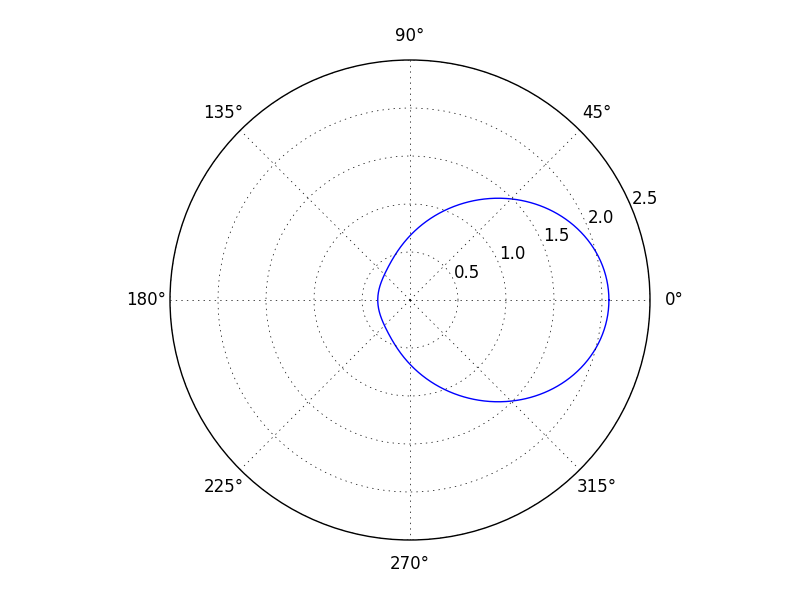
\includegraphics[width=10cm]{p5_3wave_kr1.png}
\end{center}
The total cross section is $10.6R^2$.
This should be reasonably accurate since higher partial waves doesn't contribute
much at low energy. When the wavelength is very large,
only the first partial wave is important and the scattering is symmetric.

\section{}
Let $a\equiv\dfrac{\hbar^2}{mg}$
For incident wave from left
\eqar{
  \psi=&\left\{
    \begin{array}{ll}
      \ue^{\ui kx}+r\ue^{-\ui kx}&x<0\\
      t\ue^{\ui kx}&x>0
    \end{array}
  \right.\\
  1+r=&t\\
  \frac{2}{a}t=&\ui kt -\ui k+\ui kr\\
  t=&\frac{ka}{ka+\ui}\\
  r=&\frac{-\ui}{ka+\ui}
}
For incident wave from right
\eqar{
  \psi=&\left\{
    \begin{array}{ll}
      \ue^{-\ui kx}+r'\ue^{\ui kx}&x>0\\
      t'\ue^{-\ui kx}&x<0
    \end{array}
  \right.\\
  1+r'=&t'\\
  \frac{2}{a}t'=&\ui kt' -\ui k+\ui kr'\\
  t'=&\frac{ka}{ka+\ui}\\
  r'=&\frac{-\ui}{ka+\ui}
}
The scattering matrix in the $k$ subspace.
\eqar{
  S=&\frac{1}{ka+\ui}\begin{pmatrix}
    ka&-\ui\\
    -\ui&ka
  \end{pmatrix}\\
  SS^\dagger=&\frac{1}{ka+\ui}\begin{pmatrix}
    ka&-\ui\\
    -\ui&ka
  \end{pmatrix}\frac{1}{ka-\ui}\begin{pmatrix}
    ka&\ui\\
    \ui&ka
  \end{pmatrix}\\
  =&\frac{1}{k^2a^2+1}\begin{pmatrix}
    k^2a^2+1&0\\
    0&k^2a^2+1
  \end{pmatrix}\\
  =&I
}

\end{document}
